\section{Introduction} \label{introduction}

In today's software development industry, the methodology of software development is fractured
between multiple processes.
Some companies use an ``agile" methodology, iteratively developing ideas and prototyping their
products \cite{gilb1999evolutionary}. %need a citation
Others develop according to the traditional Software Development Lifecycle (SDLC) models, requiring
extensive documentation and requirements before beginning software development \cite{Royce:1987:MDL:41765.41801}.\\
\\
These are confusing categorisations, and within each are further sub-models, such as
%citations below
\begin{itemize}
	\item ``Spiral" \cite{Boehm:1986:SMS:12944.12948}
	\item ``Extreme Programming" \cite{beck2004extreme}
	\item ``Prototyping" \cite{Alavi:1984:APA:358080.358095}
	\item ``V-Model" \cite{forsberg1995relationship}
\end{itemize}
Depending on what project, some development processes are not even suitable for some software
projects and it is thus desirable to gauge how suitable one process is compared to another.\\
\\
However, each is denoted in its own format and style, making identification and classification of processes a
confusing task. %add diagrams

\begin{figure}[ht!]
  \centering
  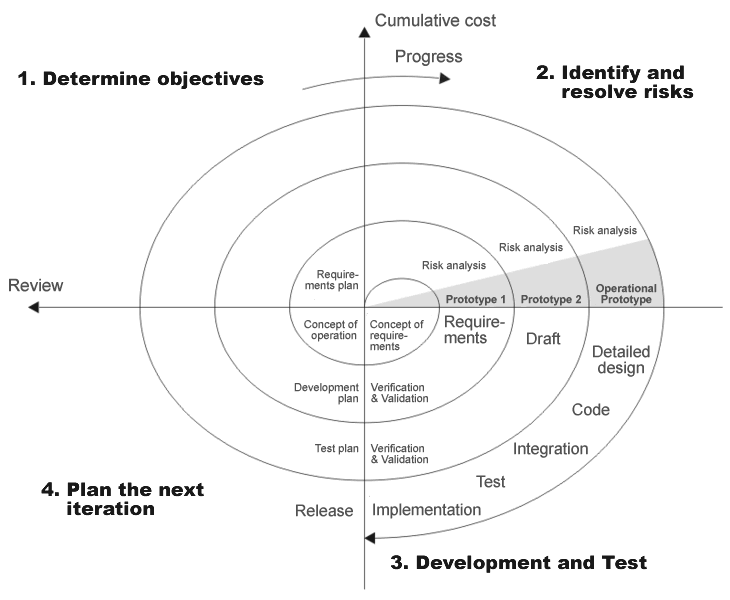
\includegraphics[scale=0.5]{media/Spiral_model_(Boehm,_1988)}
  \caption{Boehm's original Spiral model \cite{Boehm:1986:SMS:12944.12948}.}
  \label{BoehmOriSpiral}
\end{figure}

\begin{figure}[ht!]
  \centering
  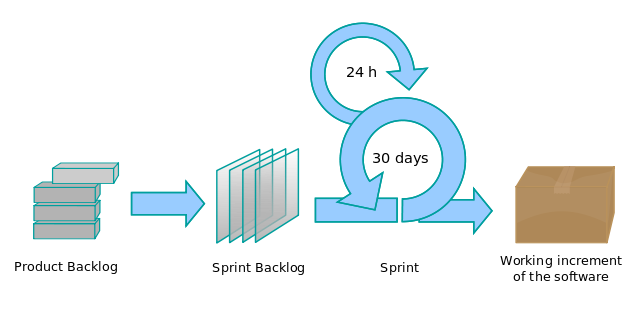
\includegraphics[scale=0.4]{media/Scrum_process}
  \caption{The Scrum model, as taken from \cite{SCRUMPIC}.}
  \label{ScrumRandomPic}
\end{figure}

\pagebreak

Comparisons about the strengths and weaknesses of each process and their suitability to fulfill a
project are thus difficult to conceive.
As an example, how could we distinguish between Figures \ref{BoehmOriSpiral} or
\ref{ScrumRandomPic} when they are denoted so differently?\\
\\
We will resolve these difficulties in by introducing a simple flow-chart based notation with some
relations to UML-activity diagrams.
We motivate the design behind our notation and why it conforms to the concepts that support a good
notation.\\
\\
We construct a taxonomy based on the distinguishing features between a set of software development
processes.
Our taxonomy will have the aim: given a software development process, which known software development process does it most
	resemble?
We will briefly touch upon another related question: given a description of informal software requirements, which known software development
	process would be suitable for its development?\\
\\
Finally, we present an analysis of the taxonomy and significant or interesting results we have
found during through the taxonomy.
We discuss what makes our taxonomy and classification system worthwhile for usage and present
conjectures about improving classification methods.
